

\tikzset{every picture/.style={line width=0.75pt}} %set default line width to 0.75pt

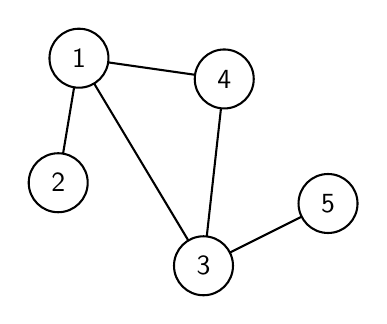
\begin{tikzpicture}[x=0.75pt,y=0.75pt,yscale=-1,xscale=1]
%uncomment if require: \path (0,181); %set diagram left start at 0, and has height of 181


% Text Node
\draw    (45, 42) circle [x radius= 14.21, y radius= 14.21]   ;
\draw (45,42) node   [align=left] {\begin{minipage}[lt]{13.600000000000001pt}\setlength\topsep{0pt}
\begin{center}
$\displaystyle \mathsf{1}$
\end{center}

\end{minipage}};
% Text Node
\draw    (115, 52) circle [x radius= 14.21, y radius= 14.21]   ;
\draw (115,52) node   [align=left] {\begin{minipage}[lt]{13.600000000000001pt}\setlength\topsep{0pt}
\begin{center}
$\displaystyle \mathsf{4}$
\end{center}

\end{minipage}};
% Text Node
\draw    (35, 102) circle [x radius= 14.21, y radius= 14.21]   ;
\draw (35,102) node   [align=left] {\begin{minipage}[lt]{13.600000000000001pt}\setlength\topsep{0pt}
\begin{center}
$\displaystyle \mathsf{2}$
\end{center}

\end{minipage}};
% Text Node
\draw    (105, 142) circle [x radius= 14.21, y radius= 14.21]   ;
\draw (105,142) node   [align=left] {\begin{minipage}[lt]{13.600000000000001pt}\setlength\topsep{0pt}
\begin{center}
$\displaystyle \mathsf{3}$
\end{center}

\end{minipage}};
% Text Node
\draw    (165, 112) circle [x radius= 14.21, y radius= 14.21]   ;
\draw (165,112) node   [align=left] {\begin{minipage}[lt]{13.600000000000001pt}\setlength\topsep{0pt}
\begin{center}
$\displaystyle \mathsf{5}$
\end{center}

\end{minipage}};
% Connection
\draw    (42.66,56.02) -- (37.34,87.98) ;
% Connection
\draw    (59.07,44.01) -- (100.93,49.99) ;
% Connection
\draw    (52.31,54.19) -- (97.69,129.81) ;
% Connection
\draw    (113.43,66.13) -- (106.57,127.87) ;
% Connection
\draw    (117.71,135.64) -- (152.29,118.36) ;

\end{tikzpicture}